\documentclass[
	12pt,
	a4paper,
	bibtotoc,
	cleardoubleempty, 
	idxtotoc,
	%ngerman,
	openright1,
	final,
	listof=nochaptergap,
	]{scrbook}

\usepackage[T1]{fontenc}
\usepackage[utf8]{inputenc}
\usepackage{longtable}
\usepackage{pdfpages}
\usepackage{babel}

% ##################################################
% Unterstuetzung fuer die deutsche Sprache
% ##################################################
\usepackage{ngerman}
\usepackage[ngerman]{babel}

% ##################################################
% Dokumentvariablen
% ##################################################

% Persoenliche Daten
\newcommand{\docNachname}{Reser}
\newcommand{\docVorname}{Christian}
\newcommand{\docStrasse}{Matthäus-Hummel-Straße 4}
\newcommand{\docOrt}{VS-Villingen}
\newcommand{\docPlz}{78050}
\newcommand{\docEmail}{christin.reser@hs-furtwangen.de}
\newcommand{\docMatrikelnummer}{256305}

\newcommand{\docNachnameZwei}{Dogan}
\newcommand{\docVornameZwei}{Yasemin}
\newcommand{\docMatrikelnummerZwei}{}

% Dokumentdaten
\newcommand{\docTitle}{Praktikumsdokumentation: Enterprise Software Architecture}
%\newcommand{\docUntertitle}{} % Kein Untertitel
\newcommand{\docUntertitle}{}
% Arten der Arbeit: Bachelorthesis, Masterthesis, Seminararbeit, Diplomarbeit
\newcommand{\docArtDerArbeit}{Dokumentation}
%Studiengaenge: Allgemeine Informatik Bachelor, Computer Networking Bachelor,
% Software-Produktmanagement Bachelor, Advanced Computer Scinece Master
\newcommand{\docStudiengang}{Informatik Master}
\newcommand{\docAbgabedatum}{30.06.2017}
\newcommand{\docErsterReferent}{Prof. Dr. Ulf Schreier}
%\newcommand{\docZweiterReferent}{-} % Wenn es nur einen Betreuer gibt
\newcommand{\docZweiterReferent}{-}

% ##################################################
% Allgemeine Pakete
% ##################################################

% Abbildungen einbinden
\usepackage{graphicx}

% Zusaetsliche Sonderzeichen
\usepackage{dingbat}

% Farben
\usepackage{color}
%\usepackage[usenames,dvipsnames,svgnames,table]{xcolor}

% Maskierung von URLs und Dateipfaden
\usepackage[hyphens]{url}

% Deutsche Anfuehrungszeichen
\usepackage[babel, german=quotes]{csquotes}

% Pakte zur Index-Erstellung (Schlagwortverzeichnis)
\usepackage{index}
\makeindex

% Ipsum Lorem
% Paket wird nur für das Beispiel gebraucht und kann gelöscht werden
\usepackage{lipsum}

% ##################################################
% Seitenformatierung
% ##################################################
\usepackage[
	portrait,
	bindingoffset=1.5cm,
	inner=2.5cm,
	outer=2.5cm,
	top=3cm,
	bottom=2cm,
	%includeheadfoot
	]{geometry}

% ##################################################
% Kopf- und Fusszeile
% ##################################################

\usepackage{fancyhdr}

\pagestyle{fancy}
\fancyhf{}
\fancyhead[EL,OR]{\sffamily\thepage}
\fancyhead[ER,OL]{\sffamily\leftmark}

\fancypagestyle{headings}{}

\fancypagestyle{plain}{}

\fancypagestyle{empty}{
  \fancyhf{}
  \renewcommand{\headrulewidth}{0pt}
}

%Kein "Kapitel # NAME" in der Kopfzeile
\renewcommand{\chaptermark}[1]{
	\markboth{#1}{}
   	\markboth{\thechapter.\ #1}{}
}

% ##################################################
% Schriften
% ##################################################

% Stdandardschrift festlegen
\renewcommand{\familydefault}{\sfdefault}
%\include{lmodern}
% Standard Zeilenabstand: 1,5 zeilig
\usepackage{setspace}
\onehalfspacing 

% Schriftgroessen festlegen
\addtokomafont{chapter}{\sffamily\large\bfseries} 
\addtokomafont{section}{\sffamily\normalsize\bfseries} 
\addtokomafont{subsection}{\sffamily\normalsize\mdseries} 
\addtokomafont{caption}{\sffamily\normalsize\mdseries} 

% ##################################################
% Inhaltsverzeichnis / Allgemeine Verzeichniseinstellungen
% ##################################################

\usepackage{tocloft}

% Punkte auch bei Kapiteln
\renewcommand{\cftchapdotsep}{3}
\renewcommand{\cftdotsep}{3}

% Schriftart und -groesse im Inhaltsverzeichnis anpassen
\renewcommand{\cftchapfont}{\sffamily\normalsize}
\renewcommand{\cftsecfont}{\sffamily\normalsize}
\renewcommand{\cftsubsecfont}{\sffamily\normalsize}
\renewcommand{\cftchappagefont}{\sffamily\normalsize}
\renewcommand{\cftsecpagefont}{\sffamily\normalsize}
\renewcommand{\cftsubsecpagefont}{\sffamily\normalsize}

%Zeilenabstand in den Verzeichnissen einstellen
\setlength{\cftparskip}{.5\baselineskip}
\setlength{\cftbeforechapskip}{.1\baselineskip}

% ##################################################
% Abbildungsverzeichnis und Abbildungen
% ##################################################

\usepackage{caption}

\usepackage{wrapfig}

% Nummerierung von Abbildungen
\renewcommand{\thefigure}{\arabic{figure}}
\usepackage{chngcntr}
\counterwithout{figure}{chapter}

% Abbildungsverzeichnis anpassen
\renewcommand{\cftfigpresnum}{Abbildung }
\renewcommand{\cftfigaftersnum}{:}

% Breite des Nummerierungsbereiches [Abbildung 1:]
\newlength{\figureLength}
\settowidth{\figureLength}{\bfseries\cftfigpresnum\cftfigaftersnum}
\setlength{\cftfignumwidth}{\figureLength}
\setlength{\cftfigindent}{0cm}

% Schriftart anpassen
\renewcommand\cftfigfont{\sffamily}
\renewcommand\cftfigpagefont{\sffamily}

% ##################################################
% Tabellenverzeichnis und Tabellen
% ##################################################

% Nummerierung von Tabellen
\renewcommand{\thetable}{\arabic{table}}
\counterwithout{table}{chapter}

% Tabellenverzeichnis anpassen
\renewcommand{\cfttabpresnum}{Tabelle }
\renewcommand{\cfttabaftersnum}{:}

% Breite des Nummerierungsbereiches [Abbildung 1:]
\newlength{\tableLength}
\settowidth{\tableLength}{\bfseries\cfttabpresnum\cfttabaftersnum}
\setlength{\cfttabnumwidth}{\tableLength}
\setlength{\cfttabindent}{0cm}

%Schriftart anpassen
\renewcommand\cfttabfont{\sffamily}
\renewcommand\cfttabpagefont{\sffamily}

% Unterdrueckung von vertikalen Linien
\usepackage{booktabs}

% ##################################################
% Listings (Quellcode)
% ##################################################

\usepackage{listings}
\lstset{
	language=java,
	backgroundcolor=\color{white},
	breaklines=true,
	prebreak={\carriagereturn},
 	breakautoindent=true,
 	numbers=left,
 	numberstyle=\tiny,
 	stepnumber=2,
 	numbersep=5pt,
 	keywordstyle=\color{blue},
   	commentstyle=\color{green},   
   	stringstyle=\color{gray}
}
  	
% ##################################################
% Theoreme
% ##################################################
  	
% Umgebung fuer Beispiele
\newtheorem{beispiel}{Beispiel}

% Grafik dynamisch zum Text mit \begin{figure}[H] - H Option ist wichtig
\usepackage{float}

% Umgebung fuer These
\newtheorem{these}{These}

% Umgebung fuer Definitionen
\newtheorem{definition}{Definition}
  	
% ##################################################
% Literaturverzeichnis
% ##################################################

\usepackage{bibgerm}

% ##################################################
% Abkuerzungsverzeichnis
% ##################################################

\usepackage[printonlyused]{acronym}

% ##################################################
% PDF / Dokumenteninternelinks
% ##################################################

\usepackage[
	colorlinks=false,
   	linkcolor=black,
   	citecolor=black,
  	filecolor=black,
	urlcolor=black,
    bookmarks=true,
    bookmarksopen=true,
    bookmarksopenlevel=3,
    bookmarksnumbered,
    plainpages=false,
    pdfpagelabels=true,
    hyperfootnotes,
    pdftitle ={\docTitle},
    pdfauthor={\docVorname~\docNachname},
    pdfcreator={\docVorname~\docNachname}]{hyperref}

\begin{document}

\setcounter{secnumdepth}{3}

% Titelblatt
\begin{titlepage}
\pagestyle{empty}

% ##################################################
% HFU-Logo einbinden
% ##################################################
\begin{flushright}
\begin{figure}[ht]
\flushright

\includegraphics[height=3cm]{content/pictures/hfu.jpg}
\end{figure}
\end{flushright}

% ##################################################
% Titel
% ##################################################
\begin{center}
{\fontsize{18}{22} \selectfont \docArtDerArbeit}\\[5mm]
{\fontsize{18}{22} \selectfont im Studiengang} \\[5mm]
{\fontsize{18}{22} \selectfont \docStudiengang}\\
\vspace{1cm}
\begin{onehalfspace}
{\fontsize{22}{26} \selectfont \textbf{\docTitle}}\\[5mm]
{\fontsize{18}{22} \selectfont \docUntertitle}


\end{onehalfspace}
\end{center}

% ##################################################
% Zusatzinformationen
% ##################################################
\vfill
\begin{center}
\begin{tabular}{lcl}
Referent  		&:& \docErsterReferent 	\\ \\
Vorgelegt am 	&:& \docAbgabedatum 	\\ \\
Vorgelegt von 	&:& \docVorname~\docNachname~\docMatrikelnummer~INM, \\
				& &	 \docVornameZwei~\docNachnameZwei~\docMatrikelnummerZwei~INM \\
	
\end{tabular}
\end{center}
\end{titlepage}
\cleardoubleemptypage

\frontmatter


% Abstract
%\chapter*{Abstract\markboth{Abstract}{}}
\addcontentsline{toc}{chapter}{Abstract}

The complexity of embedded systems in the automotive industry has increased steadily.
The developement of these complex embedded systems is very time-consuming,
therefore companies try to reuse as much of former projects as possible.
To make an efficient reuse possible, companies are in need of globally recognized standards,
whereby the automotive area originated the \ac{AUTOSAR} standard.
\ac{AUTOSAR} specifies the interfaces between features. Everything that is too specific to be standardized is covered within \textit{complex device drivers}.
\\
The scope of the bachelor thesis is a first introduction of the AUTOSAR-compliant tool \textit{EB Tresos Studio}, for the developement of configuration projects,
which allow a partial generation of complex device driver sourcecode.
\\
\\
Die Komplexität von embedded systems in der Automotive Industrie hat im Laufe der Zeit stetig zugenommen.
Die Entwicklung dieser komplexen embedded systems ist sehr zeitaufwändig, daher versucht man so viel wie möglich wiederzuverwenden.
Um eine effiziente Wiederverwendung zu ermöglichen, benötigt es weltweit anerkannte Standards, 
wodurch der Automotive Bereich den \acf{AUTOSAR} Standard ins Leben gerufen hat.
\ac{AUTOSAR} spezifiziert die Schnittstellen zwischen Features, alles was dadurch nicht abgedeckt ist, wird in \textit{Complex Device Drivern} umgesetzt.
\\
Ziel der Bachelorarbeit ist die Einführung des AUTOSAR-konformen Werkzeuges \textit{EB Tresos Studio}, für die Entwicklung von Konfigurationsprojekten, die 
eine Quellcode Generierung für Teile von Complex Device Drivern ermöglichen soll.

%\cleardoubleemptypage

% Inhaltsverzeichnis
\tableofcontents
\addcontentsline{toc}{chapter}{Inhaltsverzeichnis}
\cleardoubleemptypage

% Abbildungsverzeichnis einbinden und ins Inhaltsverzeichnis
% WORKAROUND: tocloft und KOMA funktionieren zusammen nicht
% korrekt\phantomsection
\addcontentsline{toc}{chapter}{\listfigurename} 
\listoffigures
\cleardoubleemptypage

% Tabellenverzeichnis einbinden und ins Inhaltsverzeichnis
% WORKAROUND: tocloft und KOMA funktionieren zusammen nicht
% korrekt\phantomsection
\phantomsection
\addcontentsline{toc}{chapter}{\listtablename}
\listoftables
\cleardoubleemptypage

% Abkürzungsverzeichnis
\chapter*{Abkürzungsverzeichnis\markboth{Abkürzungsverzeichnis}{}}
\addcontentsline{toc}{chapter}{Abkürzungsverzeichnis}

\begin{acronym}
 \acro{HTML}{Hypertext Markup Language}
 \acro{JPA}{Java Persistence API}
 \acro{JSF}{Java Server Faces}
 \acro{CRUD}{Create Read Update Delete}
 \acro{ORM}{Object Relational Mapping}
 \acro{UI}{User Interface}
\end{acronym}

\nocite{*}
\mainmatter

\chapter{Einführung und Ziele}

Im Rahmen des Praktikums der Lehrveranstaltung \enquote{Enterprise Software Architektur} soll eine Webapplikation
entstehen, bei der alle aktuell gängigen Technologien der Java Enterprise Edition eingesetzt werden sollen. 
Dazu gehören zuallererst die Java Server Faces (JSF), ein Framework zur Entwicklung grafischer Oberflächen in Webanwendungen. 
JSF kann durch den Einsatz von Primefaces um neue Funktionen erweitert werden. Primefaces bietet eine Demoseite\footnote{link zur demoseite} mit allen
verfügbaren Komponenten mit implementierung an, wodurch Einsteiger einen schnelleren Einstieg in die Entwicklung finden können.
Zur Persistierung der Daten soll die Java Persistance API (JPA) eingesetzt werden. JPA bietet eine Schnittstelle, um Objekte einfacher
in eine Datenbank zu Übertragen, ohne viel SQL benutzen zu müssen. Alle Entitäten, die in einer Datenbank persistiert werden müssen,
werden mit den entsprechenden Annotations versehen und mit Hilfe eines Entitätenmanagers können Objekte eines solchen Typs
mit einer Zeile Code in die Datenbank geschrieben und herausgelesen werden. Für manche Anwendungsfälle soll eine Zugriffskontrolle stattfinden,
sodass für die zu entwickelnde Applikation ein Login zur Benutzerauthentifizierung nötig ist. 



\chapter{Anwendungsdomäne - Wettbewerbsverwaltung}
Als Anwendungsdomäne wurde eine Wettbewerbsverwaltung gewählt. Im folgenden wird die Anwend


Um wie bei einer üblichen Applikation zu beginnen, wird zunächst das zu Grunde liegende Datenmodell beschrieben.
Für die Evaluation des Frameworks wurde eine Referenz-Anwendung erstellt, die die Funktionalität des Frameworks unter Beweis stellen soll.  
\section{Beschreibung}
Die zu entwickelnde Applikation soll sich nicht auf eine bestimmte Sportart beschränken. Sie soll zum Beispiel für
Fussballwettbewerbe genauso einsetzbar sein wie für Handballwettbewerbe oder Volleyballwettbewerbe. Mit Hilfe der
CRUD-Operationen(Create, Read, Update, Delete) soll es einem Benutzer möglich sein, Wettbewerbe anzulegen,
Wettbewerbe anzuzeigen, Wettbewerbe zu bearbeiten und Wettbewerbe zu löschen. Genauso sollen Mannschaften und ihre
zugehörigen Spieler angelegt, angezeigt, bearbeitet und gelöscht werden können. Der Benutzer soll Wettbewerben die
Teilnehmenden Mannschaften hinzufügen können, genauso soll er den Mannschaften ihre Spieler hinzufügen können.

\section{Anforderungen}
Die Anforderungen an das System werden in folgendem Use-Case-Diagramm zusammengefasst. Hierbei zeigen sich drei
Aktoren. Der Admin kann Datensätze anlegen, editieren, anzeigen und löschen, sowie Mannschaften den
Wettbewerben und Spieler den Mannschaften hinzufügen. Der Aktor Benutzer, kann sich lediglich alle
Datensätze anzeigen lassen. Als dritter zeigt sich der Datenbank Aktor. Dieser Aktor persistiert die Datensätze und
stellt sie zur Verfügung.


\begin{figure}[H]
	\caption{Anwendungsfall Diagramm}
	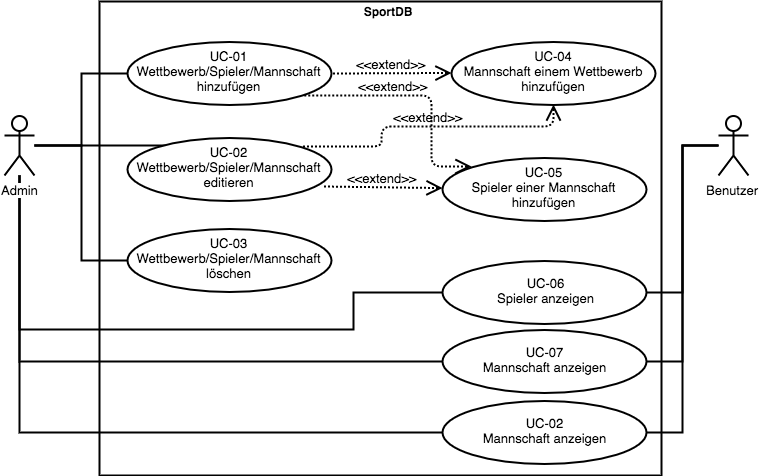
\includegraphics[width=0.9\textwidth]{content/pictures/use_case}
	\label{pic:usecase_diag}
\end{figure}

Aus den groben Anforderungen im Use-Case Diagramm kann man eine Reihe von genauen Anforderungen ableiten.
Diese sind in \ref{tab:anf_seminarverwaltung} beschrieben.


\section{Datenmodell}

Folgendes Datenmodell zu sehen in Abb. \ref{pic:datamodel} ist entstanden. Zu sehen sind die relevanten Modelklassen und ihre Abhängigkeiten zueinander. 
Diese Daten sind durch das CRUD-Framework modifizierbar. Zwischen Wettbewerb und Mannschaft besteht eine One-to-Many Beziehung, genauso wie zwischen Mannschaft und Spieler.




\begin{figure}[htb!]
	\caption{Datenmodell Klassendiagramm}
	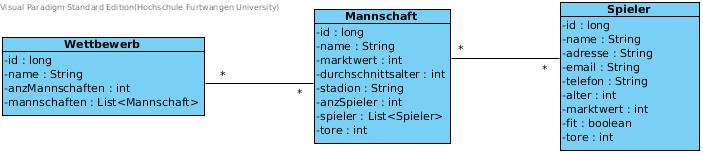
\includegraphics[width=0.9\textwidth]{content/pictures/klassendiagramm_model}
	\label{pic:datamodel}
\end{figure}



\chapter{Gesamtsystem}

\section{Komponentendiagramm}
Abbildung \ref{pic:component_diag} zeigt die fachliche Aufteilung der Softwarekomponenten. Es lassen sich drei Schichten ableiten. An oberster Stelle steht die Webapp mit den Templates 
aller Seiten und Unterseiten. Diese Templates greifen auf die Controller der Komponenten darunter zu. Jede Komponente, also wettbewerbe, mannschaften, spieler und login beinhalten ihre 
eigenen Controller in einem Controller Paket. Ausser dem Controller Paket befindet sich noch ein Paket für die Modelklassen, ein Paket für die Producer, welche Objekte erzeugen die injected werden 
können und ein Servicepaket zur Kommunikation mit der Datenbank jeder Komponente. Die unterste Schicht, die persistance Komponente schreibt und liest Daten aus einer H2 Datenbank mit Hilfe 
des JPA-Frameworks. 




%In der Abbildung \ref{pic:component_diag} ist die Übersicht der Systembausteine dargesstellt. 
%Das System selbst ist in drei Schichten aufgeteilt. Eine Schicht, für die Benutzeroberfläche, die Steuereinheiten und Oberflächenelemente enthält.
%Eine Schicht für das Datenmodell und eine Schicht für die Daten-Persistenz.\\
%\\
%Innerhalb der Schichten, gibt es zwei rot markierte Komponenten. Die \enquote{ObjectTemplate-Komponente} und  die \enquote{DataModel-Komponente}. 
%Diese stellen die Elemente dar, die an den spezifischen Anwendungsfall angepasst werden müssen. 
%Die \enquote{Datamodel}-Komponente entspricht dem tatsächlichen Datenmodel der Anwendung. 
%Alle Elemente, die vom Framework dargestellt werden sollen, müssen das Viewable-Interface aus der \enquote{AbstractModel}-Komponente implementieren.
%Zusätlich müssen für alle Elemente des Datenmodells eigenene Frontend-Template erstellt werden, welche ein bestimmtes Namensschema befolgen - Die \enquote{Object-Templates}. 
%Ein einheitliches Namensschema löst das Problem mit unterschiedlichen Darstellungsmöglichkeiten. Innerhalb der Templates ist es möglich 
%Validierungskriterien für die Element-Attribute zu formulieren, wodurch die Konsistenz des Datenbestandes gesichert werden soll.\\
%\\
%Die Steurungselemente des User-Interfaces, sowie die Templates, arbeiten mit
%den Elementen der \enquote{AbstractModel}-Komponente. Dies ermöglicht einen Austausch des Datenmodels der Anwendung. 
%Damit der Datenbestand persistiert werden kann, setzt das Framework voraus, dass jedes Viewable-Element eine Entity des JPA-Frameworks ist. Das \enquote{Loader}-Element der \enquote{Controller}-Komponente 
%greift direkt auf das JPA zu, um die Daten in der Datenbank zu verwalten. Es arbeitet jedoch immer nur mit den \enquote{Viewable}-Elementen. 

%Für die Formatierung der Abbildung -> newpage -> sonst springt es wohin es will.
%\newpage

\begin{figure}[H]
	\caption{Komponenten Diagramm}
	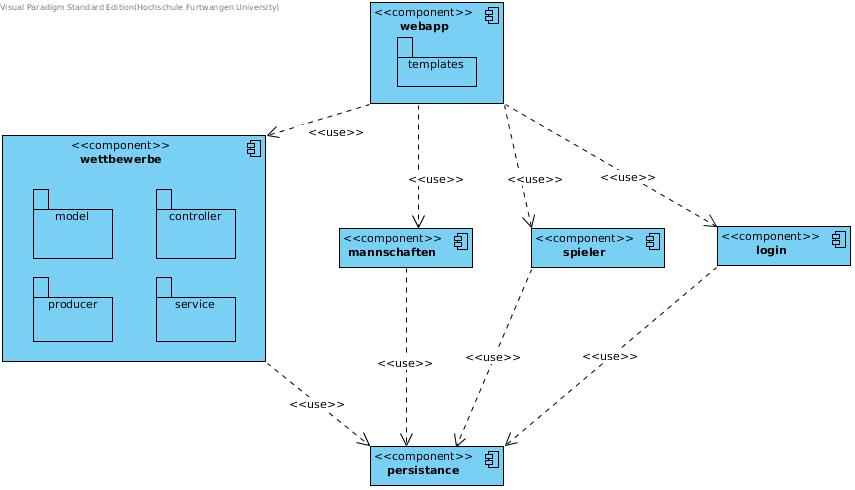
\includegraphics[width=0.9\textwidth]{content/pictures/komponentendiagramm}
	\label{pic:component_diag}
\end{figure}

%Die Abbildung \ref{pic:concrete_component_diag} zeigt das Gesamtsystem im Kontext aller extern verwendeten Komponenten.
%Die Benutzeroberfläche basiert auf der Primefaces Technologie. Der \acs{JSF}-Ansatz erlaubt ein Template basiertes arbeiten und ermöglicht somit einen
%hohen Grad der Wiederverwendbarkeit. Es kam die \acs{JSF}-Erweiterung \enquote{Primefaces} zum Einsatz, welche vorgefertigte UI-Elemente
%bereitstellt, um einen möglichst schnellen Fortschritt zu ermöglichen. Der \acs{JSF}-Ansatz ist webbasiert und benötigt deswegen einen Applikation-Server.
%In dem System wird der Glassfish4-Server eingesetzt. Obwohl der Support abgestellt wurde, bietet er eine sehr gute Referenzimplementierung.
%Für ein Logging von Ereignissen innerhalb des Systems wurde \enquote{log4j} verwendet.\\
%\\
%Auf der untersten Ebene des Systems ist die Datenpersistenz, welche über \acs{JPA} umgesetzt wurde. Es wird darunter die Datenbank H2, wegen ihrer
%Schlankheit eingesetzt. Das Datenmodell kommuniziert über die JPA-Annotationen mit der Datenbank. Während es in der UI-Schicht einen Kontroller gibt,
%welcher die expliziten Datenbankzugriffe und die Kommunikation mit der Benutzerobefläche regelt.

\begin{figure}[H]
	\caption{konkrete externe Komponenten}
	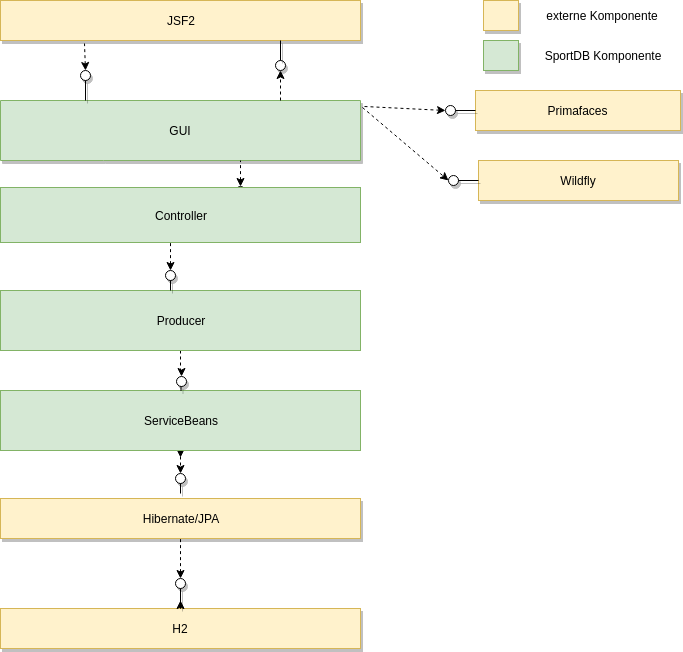
\includegraphics[width=0.9\textwidth]{content/pictures/externdiagram}
	\label{pic:concrete_component_diag}
\end{figure}



\chapter{Systembechreibung}

\section{Lösungsstrategie}

\subsection{Templates}


\subsection{Controller}

\subsection{Producer}

\subsection{ServiceBeans}

\subsection{JPA}





Die Grundidee hinter dem Framework basiert auf dem Gedanken, dass alle simplen \acs{CRUD}-Anwendungen ein gleiches Verhalten aufweisen, da sie die selbe Funktionalität
zur Verfügung stellen, nämlich \textit{Lesen, Schreiben, Löschen und Ändern}.
Wenn man eine weitestgehend individuelle Benutzeroberfläche außer Acht lässt, liegt der einzige Unterschied zwischen den Anwendungen im Inhalt und der Bedeutung der Datenmodelle.
Darauf basierend braucht es auch an das Datenmodel angepasste Darstellungen in der Benutzeroberfläche.
Das CRUD-Framework geht davon aus, dass ein Datenmodel einer \acs{CRUD}-Anwendung aus drei Komponenttypen besteht. 
Die \enquote{Viewable}-Komponenten, die im Normalfall den Klassen des Datenmodels und den JPA-Entities. 
Die \enquote{ModelLists}, die Sammlungen von Viewable-Komponenten darstellen. 
Die \enquote{Associations}, die eine Erweiterung der ModelList sind. Sie bilden die Beziehungen zwischen den einzelnen Datenmodel-Elementen.\\
\\
Diese abstrakte Darsellung der Datenmodel-Elemente ist ausreichend um die gesamte Funktionalität einer CRUD-Anwendung abbilden zu
können. Diese Eigenschaft macht sich das \acs{CRUD}-Framework zu nutze. Ein Anwender muss nur noch die definierte Schnittstelle in sein Datenmodel implementieren und 
passende XHTML-Temlates für die Darstellung der Elemente erstellen.

\section{Anforderungen}

Das Framework muss in der Lage sein ein Datenmodell und dazugehörige Templates im XTHML Format entgegen zunehmen und eine funktionierende
CRUD-Applikation daraus zu machen. Das Framework soll die gesamte Steuerung der Applikation übernehmen, indem es eine
Reihe von Steuereinheiten und Interfaces zur Verfügung stellt. Einer der Hauptansprüche des Systems, ist eine
automatische Erkennung der Relationen zwischen den Datenmodellen und die richtige Abbildung derer.
Desweiteren sind Hauptanforderungen an das Framework eine Schnittstelle für Fehlermeldungen und Logging. 
Die Daten werden vom System mittels JPA persistiert, sofern das Datenmodell JPA-Entitäten implementiert.

\section{Datenmodel des Frameworks}

In den vorhergehenden Kapiteln wurden das Datenmodel des Frameworks bereits erläutert. Die Datenstruktur ist in der Abbildung
\ref{pic:guimodel} dargesstelt. Dieses besteht aus drei Elementen:\\



\begin{figure}[htb!]
	\caption{GUI-Modell Klassendiagramm}
	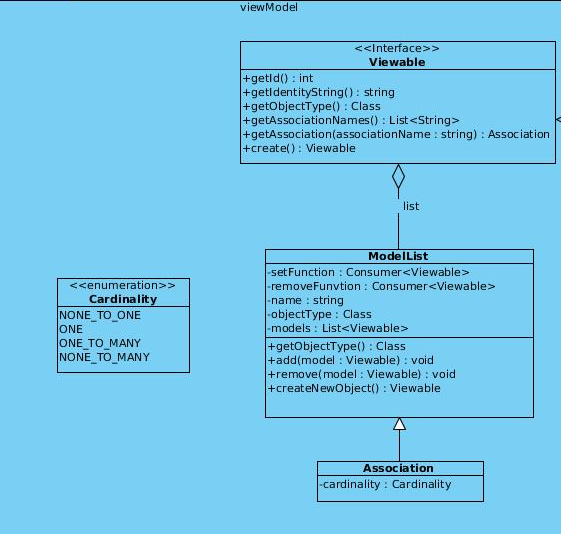
\includegraphics[width=0.9\textwidth]{content/pictures/Guimodel}
	\label{pic:guimodel}
\end{figure}

\section{Templates}
Als Templates werden die XHTML-Vorlagen bezeichnet. Diese können in zwei Gruppen aufgeteil werden: Object-Templats und Service-Templates.
Die Object-Templates werden für die Darstellung der einzelnen Viewable-Objekte verwendet. Diese müssen einem bestimmten Namenschema folgen, welches
den Klassenname beinhaltet. Der Inhalt der Objekt-Templates kann abhängig vom Anwendungsfall angepasst werden. Die einzelnen Elemente 
dieser Templates können zusätliche Validierungskriterien beinhalten.\\
\\
Die Templates sind durch Kompositionen miteinander verknüpft. 
Die Applikation beginnt in der Hauptansicht dem Index-Template, von welcher man in vier Listenansichten gelangt. In einer Listenansicht, 
kann man ein neues Objekt erzeugen, ein vorhandenes Objekt bearbeiten bzw. löschen, oder einfach einsehen. Wenn man ein Objekt löscht, so bleibt man in der Listenansicht - 
In jedem anderen Fall gelangt, man in die Objektansicht.
Jede Objektansicht besitzt Referenzen auf andere Objekte, also Assoziationen. Diese Referenzen, werden in der Objektansicht ebenfalls 
gezeigt. Wenn man diese Referenz einsehen will, so gelangt man immer zunächst in die Listenansicht der angeforderten Objekte, 
auch wenn nur ein Objekt vorhanden ist.
\\
Die Service-Templates verwenden nur die Objekte der \enquote{AbstractModel}-Komponente und können nach Bedarf Object-Templates einbinden.
Es gibt folgende Service-Templates:\\
\begin{description}
\item[Index-Template] 
Ist das Template für die Hauptseite der Benutzeroberfläche. Es beinhaltet die \enquote{Sidebar} der Anwendung. Zusätzlich enthält es das \enquote{Contentpane} der Anwendung, in dem andere 
Templates eingefügt werden können. In Abbildung \ref{pic:semVer_allViews} sieht man eine Repräsentation der Hauptansicht der integrierten Listenansicht und einer Objektansicht.
\item[ListView]
Ist das Template für die Listenansichten. Es wird für die Darstellung der ModelList bzw. Association verwendet. Eine ListView beinhaltet immer zugehörige Object-Templates, da
man einzelne Objekte innerhalb der Listenansicht ebenfalls ansehen kann.
\item[NewView]
Das Tempalte wird bei der Ertellug eines neuen Objekts verwendet. Es bindet die zugehörigen Object-Templates sowie das SelectView-Template ein.
\item[SelectView]
Dieses Template wird verwendet wenn existierende Objekte zu einer Assoziation hizugefügt werden sollen. Ein Beispiel sieht man in Abbildung \ref{pic:semVer_selectView}
\item[LogInView]
Ein Template, welches für die Benutzerauthentifizierung verwendet wird. Die dazugehörige Umsetzung sieht man in Abbildung \ref{pic:semVer_loginView}
\end{description}


\begin{figure}[htb!]
	\caption{Templates Screenshot}
	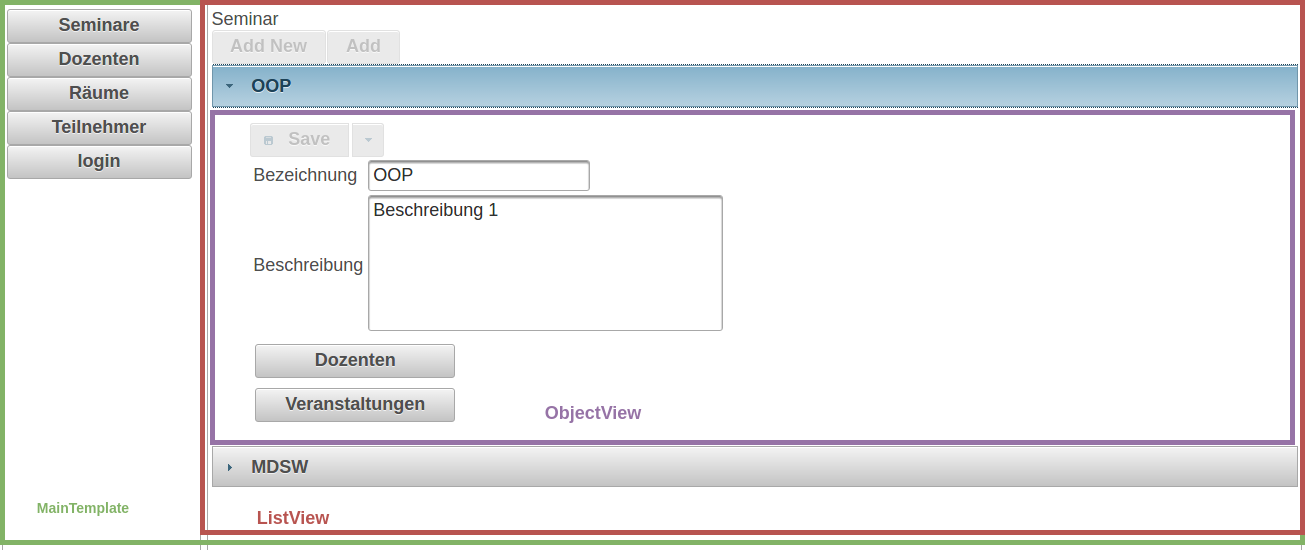
\includegraphics[width=0.9\textwidth]{content/pictures/Seminarverwaltung_ListAndObjectView}
	\label{pic:semVer_allViews}
\end{figure}

\begin{figure}[htb!]
	\caption{LoginView Screenshot}
	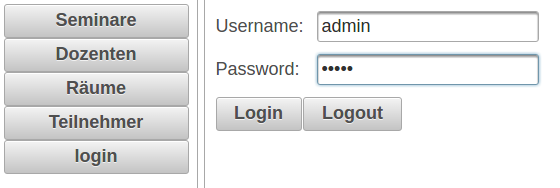
\includegraphics[width=0.9\textwidth]{content/pictures/Seminarverwaltung_LoginView}
	\label{pic:semVer_loginView}
\end{figure}

\begin{figure}[htb!]
	\caption{SelectView Screenshot}
	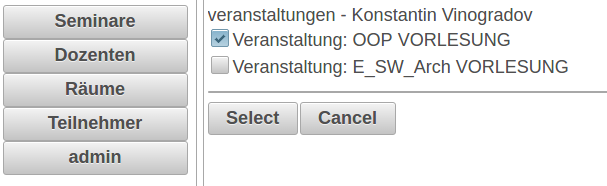
\includegraphics[width=0.9\textwidth]{content/pictures/Seminarverwaltung_SelectView}
	\label{pic:semVer_selectView}
\end{figure}

\newpage

\section{Controller}

Die Controller-Komponenten können, mit der Ausnahme des MainController, in zwei Gruppen aufgeteilt werden: UI- und Service-Controller.
Die UI-Controller sind für die Funktionalität einzelner Ansichten zuständig. Die Serivce-Controller regeln den Datenbankzugriff,
Fehlerbehandlung und Logging.

\subsection{MainController}
Der MainController nimmt eine Sonderrolle ein. Er dient als Kommunikations-Knotenpunkt und bestimmt welcher UI-Controller die Steuerung 
übernehmen soll. Dies ist die Hauptsteuereinheit, weswegen sie alle anderen Steuereinheiten kennt und deligiert. Zusätzlich steuert sie,
welches Template gerade sichtbar ist.

\subsection{UI-Controller}

Diese Steuereinheiten sind rein für die Verwaltung und Kommunikation der Benutzeroberfläche verantwortlich.
Die drei wichtigsten Steuereinheiten sind der \enquote{ListViewController}, \enquote{SelectViewController} und \enquote{NewViewController},
die ausführlicher erläutert werden.

\paragraph{ListViewController}

Der ListViewController ist für die Verwaltung der Listenansicht zuständig. Der MainController überträgt ihm die Kontrolle
nachdem mit dem Loaderkommuniziert wurde, um die benötigten Daten aus der Datenbank zu laden.\\
\\
Der typische Ablauf für diese Steuereinheit ist das Anzeigen einer Liste. 
Der Ablauf bei der Erstellung der Listenansicht ist in dem Diagramm \ref{pic:showListSeq_diag} dargestellt. Dabei bindet 
das ListView-Template zugehörige Objekt-Templates zur Laufzeit ein. Die Datenobjekte und die Information, ob der Nutzer
die Daten bearbeiten darf, werden bei der Anbindung übergeben. Eine Typprüfung der Datenobjekte findet nicht statt.

\begin{figure}[htb!]
	\caption{ShowList Sequenzdiagramm}
	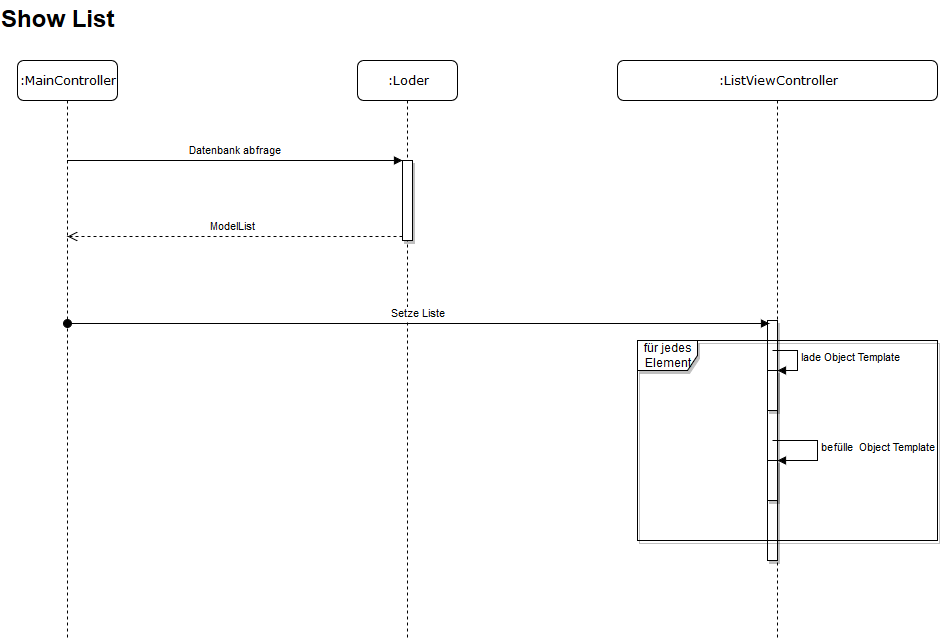
\includegraphics[width=0.9\textwidth]{content/pictures/ShowListSeq}
	\label{pic:showListSeq_diag}
\end{figure}

\paragraph{SelectViewController}
Der SelectViewController ist für die Zuordnung von existierenden Objekten zu anderen Objekten zuständig. Er ermöglicht z.B.,
dass in diesem generischen Ansatz ein Teilnehmer einer Veranstaltung zugeordnet werden kann.\\
\\
Die Select Funktionalität wird von der Listenasicht zur Verfügung gestellt. Sie wird nur für die Assoziationsdarstellung benötigt. 
Der Ablauf ist in dem Diagramm \ref{pic:selectSeq_diag} dargestellt. Zu vermerken ist, dass die Validerung der Auswahl anhand der
Kordinalität seiner Assoziation, nicht unter die Aufgaben des SelectViewControllers fällt.  

\begin{figure}[htb!]
	\caption{Select Sequenzdiagramm}
	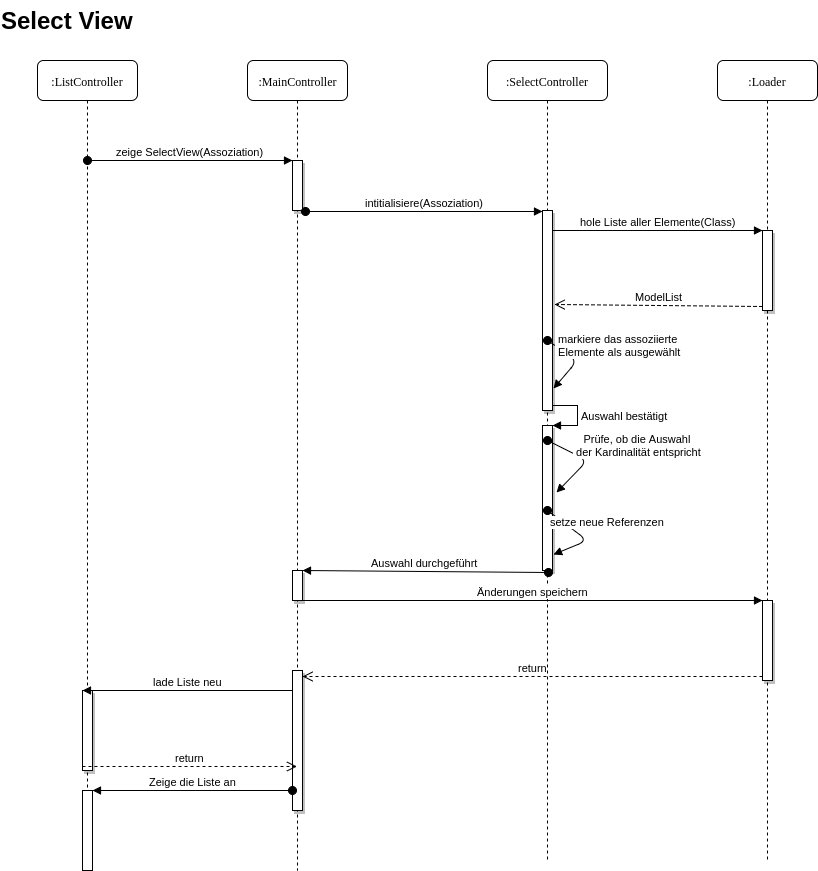
\includegraphics[width=0.9\textwidth]{content/pictures/SelectSeq}
	\label{pic:selectSeq_diag}
\end{figure}



\paragraph{NewViewController}
Der NewViewController ist für die korrekte Erzeugung und Zuordung eines neu angelegten Objektes und seiner Abhängigkeiten verantwortlich.
\\
\\
Das Diagramm \ref{pic:createNewViewSeq_diag} stellt die Kommunikation zwischen den Controller-Elementen bei der Erstellung eines neun
Datenobjekts dar. Der Vorgang kann aus der ListView ausgelöst werden. Der Ablauf unterscheidet sich abhängig davon, ob es sich bei
dem Ausgangselement um eine \enquote{ModelList} oder eine \enquote{Association} handelt. Bei einer Association kann das Datenobjekt automatisch bei der Erstellung gestzt
werden.

\begin{figure}[H]
	\caption{CreateNewView Sequenzdiagramm}
	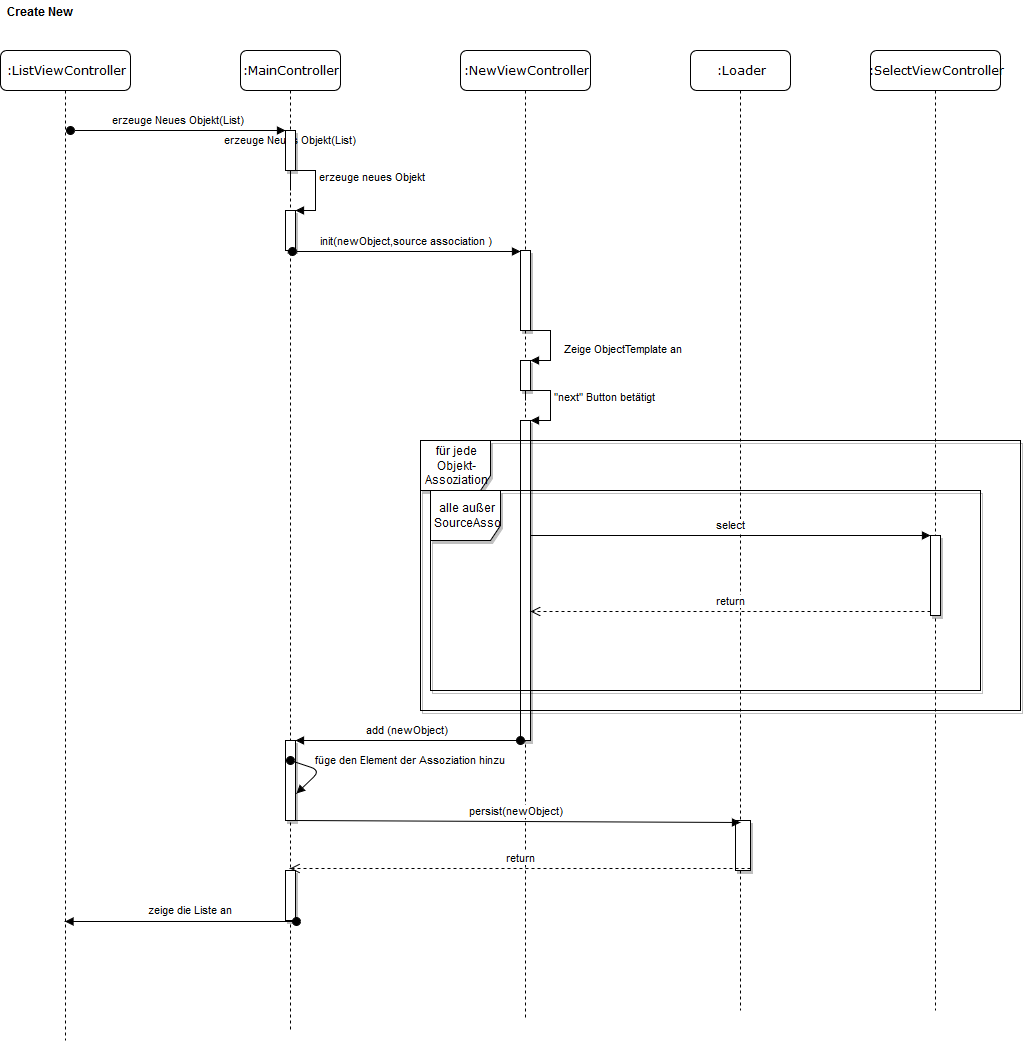
\includegraphics[width=0.9\textwidth]{content/pictures/CreateNewView}
	\label{pic:createNewViewSeq_diag}
\end{figure}

\paragraph{UserLoginController}
Der UserLoginController regelt die Zugriffsrechte im System und ist für den gesamten Login-Vorgang verantwortlich.\\
\\
Wenn ein Benutzer sich am System anmelden will, so gibt er seine Nutzerdaten ein. Diese Steuereinheit sucht nach dem Nutzernamen und
entschlüsselt das AES verschlüsselte Passwort, um es mit der Eingabe abzugleichen. Sollte der Vorgang erfolgreich sein, wird ein
globaler Flag umgeswitcht, welcher die Bearbeitungsfunktionalität freischält.

\subsection{Service-Controller}

Die Service-Controller werden von anderen Controllern verwendet, werden aber nicht direkt aus der UI angesprochen.
Es gibt die folgenden zwei Service-Controller:\\

\paragraph{MessagesViewController}
Der MessagesViewController ist ein Wrapper für unsere Logging-Komponente \enquote{log4J}. Es bietet die Möglichkeit alle Ereignisse
an zentraler Stelle zu verwalten und ermöglicht gleichzeitig die Kommunikation mit dem Nutzer, über diverse Anzeigen, die Primefaces
zur Verfügung stellt.

\paragraph{Loader}

Der Loader übernimmt die Kommunikation mit der Datenbank. Er hält einen EntityManger und \acs{CRUD}-Funktionalität für die Datenbank.
Zusätzlich enthält diese Steuereinheit den Datenbank-Treiber, welcher benötigt wird, da wir uns für eine lokale Datenbank entschieden haben
und \acs{JPA} dann keine automatische Konfiguration vornehmen kann.



%\chapter{Laufzeitsicht}
In diesem Kapitel werden die Abläufe zwischen den Controllern erklärt. Es wird auf die Teile der Controller-Kommunikation eingegangen, 
die einer expliziten Erläuterung bedürfen.
\section{Select}

\begin{figure}[htb!]
	\caption{Select Sequenzdiagramm}
	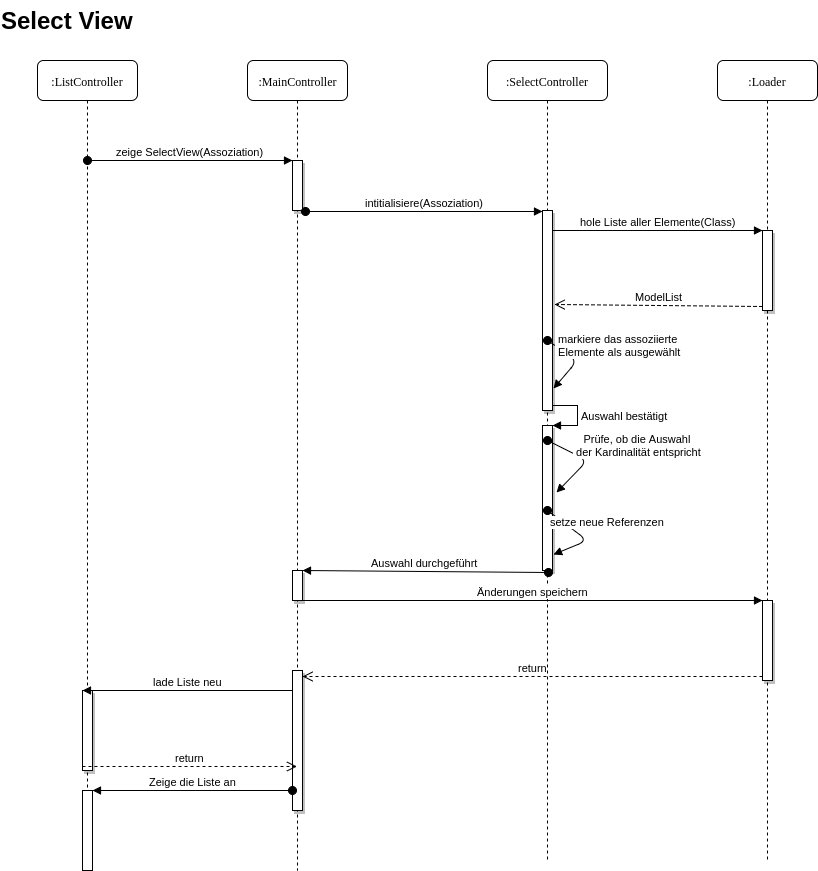
\includegraphics[width=0.9\textwidth]{content/pictures/SelectSeq}
	\label{pic:selectSeq_diag}
\end{figure}

Die Select Funktionalität wird von der Listenasicht zur Verfügung gestellt. Sie wird nur für die Assoziationsdarstellung benötigt. 
Der Ablauf ist in dem Diagramm \ref{pic:selectSeq_diag} dargestellt. Zu vermerken ist, dass die Validerung der Auswahl anhand der
Kordinalität seiner Assoziation, nicht unter die Aufgaben des SelectViewControllers fällt.  

\section{ShowList}

\begin{figure}[htb!]
	\caption{ShowList Sequenzdiagramm}
	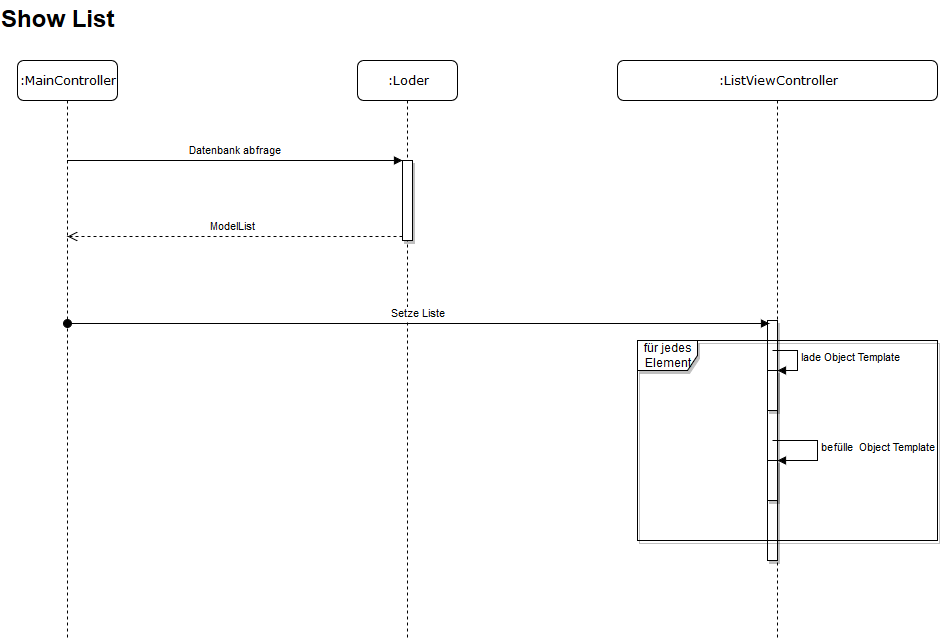
\includegraphics[width=0.9\textwidth]{content/pictures/ShowListSeq}
	\label{pic:showListSeq_diag}
\end{figure}

Der Ablauf bei der Erstellung der Listenansicht ist in dem Diagramm \ref{pic:showListSeq_diag} dargestellt. Dabei bindet 
das ListView-Template zugehörige Objekt-Templates zur Laufzeit ein. Die Datenobjekte und die Information, ob der Nutzer
die Daten bearbeiten darf, werden bei der Anbindung übergeben. Eine Typprüfung der Datenobjekte findet nicht statt.

\section{CreateNewView}

Das Diagramm \ref{pic:createNewViewSeq_diag} stellt die Kommunikation zwischen den Controller-Elementen bei der Erstellung eines neun
Datenobjekts dar. Der Vorgang kann aus der ListView ausgelöst werden. Der Ablauf unterscheidet sich abhängig davon, ob es sich bei
dem Ausgangselement um eine \enquote{ModelList} oder \enquote{Association} handelt. Bei einer Association kann das Datenobjekt automatisch bei der Erstellung gestzt
werden.

\begin{figure}[H]
	\caption{CreateNewView Sequenzdiagramm}
	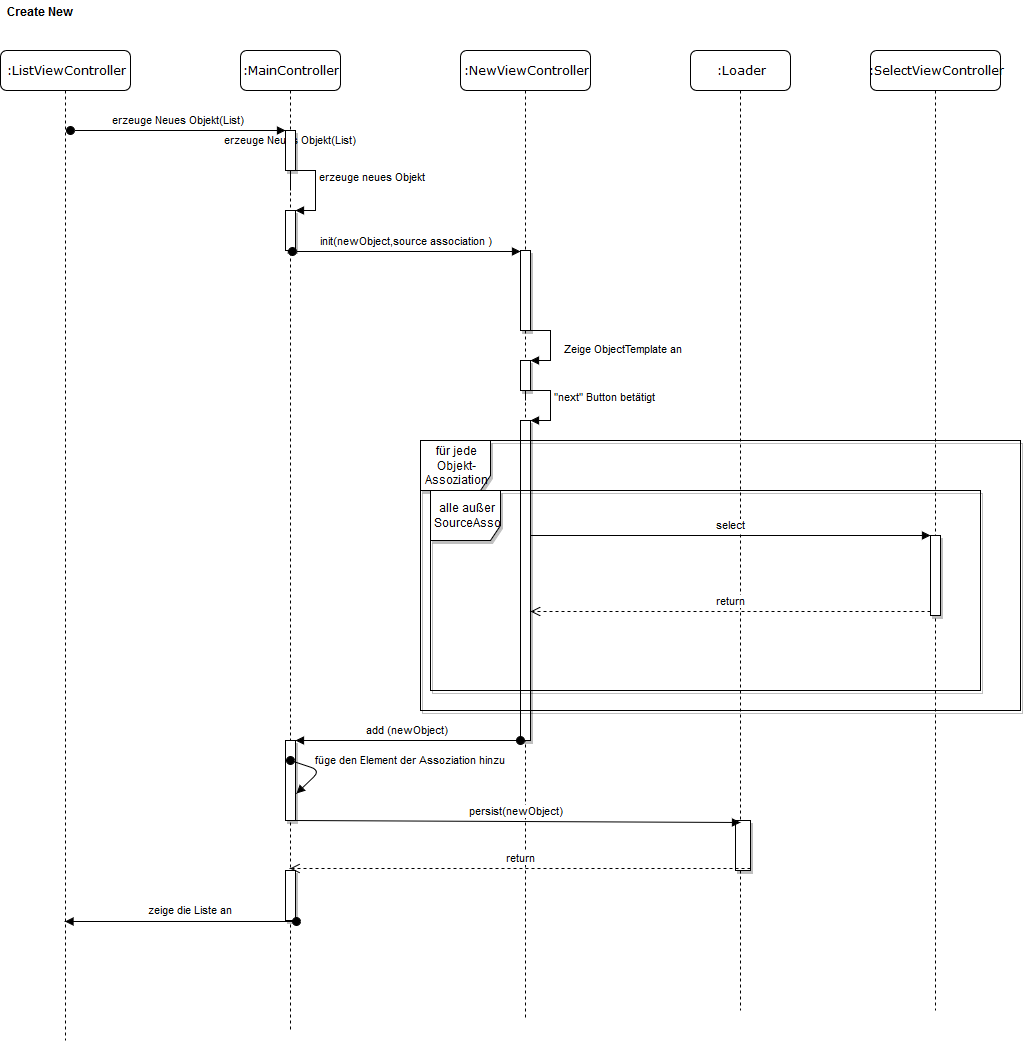
\includegraphics[width=0.9\textwidth]{content/pictures/CreateNewView}
	\label{pic:createNewViewSeq_diag}
\end{figure}


\chapter{Ergebnis}

\section{Anforderungen}

\section{Elemente}

\subsection{Datensätze anzeigen}

\subsection{Datensätze anlegen}

\subsection{Datensätze bearbeiten}

\subsection{Datensätze löschen}

%\begin{footnotesize}
%	\begin{longtable}[l]{|p{3,0cm}| p{10,5cm} |}
%		\caption{Entwurfsentscheidungen}
%		\label{tab:gui_model_desc}
%		\hline
%		\textbf{Primefaces} &
%		Eine der Vorgaben war es mit \acs{JSF} zu arbeiten. Primefaces ist eine Erweiterung der \acl{JSF} um UI-Elemente und Valiedierungsmechanismen.
%		\hline
%		\textbf{Maven} & 
%		Maven ist heutzutage ein sehr gängiges und auch praktisches Werkzeug um Projekt-Abhängigkeiten dynamisch und automatisch herunterzuladen und einzubinden.
%		\hline
%		\textbf{SinglePage Applikation} &
%		Der Kompositionslastige Aufbau einer \acs{CRUD}-Anwendung hat die Entscheidung ein Stück weit abgenommen, da die einzelnen Templates ebenfalls nur als
%		Komposition in immer allgemeineren Templates sind. Zusätzlich ist eine solche Ansicht intuitiv und benutzerfrundlich.
%		\hline
%		\textbf{JPA} &
%		\ac{ORM} Frameworks sind heutzutage Gang und Gebe. \acs{JPA} ist hierbei ein Java EE eigenes \acs{ORM}, welches die Persistierung von Datenbeständen erheblich vereinfacht.
%		Ein Vorteil ist zusätzlich, dass die darunterliegende tatsächliche Datenbank ausgetauscht werden kann. Wir haben uns für eine H2 Datenbank wegen seiner Schlankheit entschieden.
%		\hline	
%		\textbf{ManagedBean} &
%		Wir haben unser System auf die \enquote{@Named} Annotation umgestellt und festgestellt, dass die Ladezeiten des Systems in der Initialisierungsphase bis zu fünf Sekunden in Anspruch nehmen können.
%		Mit hoher Wahrscheinlichkeit, hat es mit irgendeiner Konfiguration unseres Systems zu tun. Allerdings wurden wir nach langem Suchen nicht fündig und haben uns für die
%		ManagedBeans entschieden, die in unserem System eine sehr viel bessere Performance erbringen.
%		\hline
%		\end{longtable}
%\end{footnotesize}
\chapter{Erweiterungsmöglichkeiten}

Eine möglich Erweiterung des Frameworks wäre eine Änderung der Schnittstelle. Anstatt wie bisher ein definiertes Interface anzubieten,
könnte man die einzelnen Interface Funktionen auch als Annotationen umsetzen. Eine Klasse im Datenmodell müsste dann die Klasse mit einer
Annotation versehen, die zeigt, dass diese in der Benutzeroberfläche angezeigt werden soll. 
Zusätzlich gäbe es eine Annotation, die über den Assoziationen innerhalb der Klasse steht. Die passenden Setter und Getter Methoden, die in der
ModelList benötigt werden, wären über Reflection zugänglich. Der Typ der Klasse wäre über Reflection ebenfalls einfach zu erhalten.
Diese Erweiterung nimmt dem Nutzer des Frameworks mehr Arbeit ab. Er muss lediglich die Assoziationen und die Klasse mit Annotationen versehen, anstatt
Kenntnis über ein Interface zu haben.\\
\\
Eine weitere Erweiterungsmöglichkeit, ist die automatische Generierung von Templates. Basierend auf dem Quellcode müsste irgendwo hinterlegt sein,
wie ein Datentyp interpretiert werden soll. Beispielsweise ist ein Boolean eine Checkbox, ein Datum ein Date-Element und ein String ein Textfeld.
Diese Erweiterung ist allerdings recht restriktiv gegenüber der Benutzerobefläche, alternativ könnte man dem Nutzer die Möglichkeit geben über spezielle 
Annotationen zu bestimmen auf welche Weise ein Attribut abgebildet werden soll. Alledings ist auch dies mit Restrktionen verbunden - Man gewinnt jedoch an Effizienz, da
nun nur noch das Datenmodell implementiert werden muss.


\chapter{Fazit}

Es sollte eine Applikation basierend auf den gängigen Java EE Features umgesetzt werden.
Hierbei wurden die Technologien \ac{JPA} und \acs{JSF} eingesetzt. Die grobe Anforderungen war es ein \enquote{größeres} Projekt umzusetzen.
Wir haben uns die Gemeinsamkeiten einer \acs{CRUD} Applikation angesehen und ein kleines Framework geschrieben, dass recht universell
auf eine große Menge an Anwendungen passt und somit Zeit erspart.\\
\\
Java EE hat einige nützlich Features, die es sich durchaus lohnt zu kennen und einmal angewendet zu haben. So ist \acs{JSF} mit den vorhandenen Erweiterungen
eine gute Methode um sehr schnell eine Anwendung mit grafischer Benutzeroberfläche umzusetzen. \acs{JPA} hingegen ermöglicht eine sehr einfache und vor allem
dynamische Methode um Daten zu persistieren. 


% Schlagwortverzeichnis (Index)
%\printindex

% Literaturverzeichnis
%\singlespacing
%\bibliographystyle{alphadin}
%\bibliography{bibtex}

% Eidesstattliche Erklärung
%\chapter*{Eidesstattliche Erklärung\markboth{Eidesstattliche Erklärung}{}}
% Eintrag in das Inhaltsverzeichnis 
\addcontentsline{toc}{chapter}{Eidesstattliche Erklärung}

Ich versichere, dass ich die vorstehende Arbeit selbständig verfasst und hierzu
keine anderen als die angegebenen Hilfsmittel verwendet habe. Alle Stellen der Arbeit die 
wörtlich oder sinngemäß aus fremden Quellen entnommen wurden, sind als solche kenntlich gemacht.
\\
\\
Die Arbeit wurde bisher in gleicher oder ähnlicher Form in keinem anderen
Studiengang als Prüfungsleistung vorgelegt oder an anderer Stelle
veröffentlicht.
\\
\\
Ich bin mir bewusst, dass eine falsche Erklärung rechtliche Folgen haben kann.

\vspace*{1.5cm} \par
\line(1,0){200} \par
\docOrt, den  \docAbgabedatum ~~\docVorname~\docNachname

\appendix
% Hier können Anhaenge angefuegt werden
%\includepdf[pages=-]{content/appendix/template_plugin_xml}
%\label{lab:template_plugin_xml}
\end{document}      